
\documentclass[runningheads]{llncs}
\usepackage{graphicx}
\usepackage{amsmath,amssymb} % define this before the line numbering.
\usepackage{lineno}
\usepackage{color}
\usepackage{multirow}
\usepackage{subfigure}
\begin{document}
\renewcommand\thelinenumber{\color[rgb]{0.2,0.5,0.8}\normalfont\sffamily\scriptsize\arabic{linenumber}\color[rgb]{0,0,0}}
%\renewcommand\makeLineNumber {\hss\thelinenumber\ \hspace{6mm} \rlap{\hskip\textwidth\ \hspace{6.5mm}\thelinenumber}}
%\linenumbers
\pagestyle{headings}
\mainmatter
\def\IVS16SubNumber{***}  % Insert your submission number here

\title{RPN-based Real-Time Vehicle Detection in Satellite Images} % Replace with your title

%\titlerunning{IVS-16 submission ID \IVS16SubNumber}

%\authorrunning{IVS-16 submission ID \IVS16SubNumber}

\author{Jingao Hu}
\institute{Institute of Automation, Chinese Academy of Sciences \newline Beijing 100190, China
}


\maketitle

\begin{abstract}
Detecting small-sized targets like vehicles in high resolution satellite images is a significant but challenging task. In the past decade, some detection frameworks have been proposed to solve this problem and made certain progress. However, like the traditional ways of object detection in natural images those methods all take multiple stages. Region proposals are first produced by some methods like selective-search, BING, then fed into the feature extractor and classified finally. Multi-stage detection schemes are designed complicated and time consuming. In this paper, we propose a single-stage remote sensing vehicle detection framework using region proposal networks (RPN). We elaborate our RPN architecture considering the trade-off between accuracy and speed and design our vehicle object-oriented training methodology in experiments. Comparison results demonstrate that our method can achieve a real time detection with comparable detection accuracy compared to state-of-the-art methods.
\end{abstract}


\section{Introduction}


Recent advances in remote sensing imagery make high-resolution satellite images more accessible. Detecting vehicle objects in those satellite images becomes an essential and meaningful research field for it can provide important information for homeland surveillance, intelligent transportation planning, disaster search and rescue, etc. . Although a lot of works have been done, there is no one that takes efficiency, robustness and speed all in consideration.

Machine learning methods are widely utilised in the research of satellite image vehicle detection in the past decade. Like traditional object detection frameworks in natural images those methods mainly take three stages. Region proposals(latent candidates) are first produced by certain proposal extracting algorithm like slective search, BING, then fed into the feature extractor and classified finally. Zhao and Nevatia\cite{t_zhao} take vehicle detection as a 3D object recognition problem so they select the boundary of the car body, front windshield and the shadow as features which are then integrated by a Bayesian network. Eikvil et al.\cite{eikvil} utilise satellite image information like road information, geometric-shape properties to assist their Hu moment-based detection method. Liang et al.\cite{p_liang} propose a detection scheme that uses multiple kernel SVM (MKL-SVM) with HOG and Haar features. They trained MKL-SVM to learn an optimal kernel with many base kernels in order to get the trade-off between HOG and Haar features. Kembhavi et al.\cite{kembhavi} construct an vehicle detection framework by extracting HOG, color probability maps and pairs of pixel as features and using a partial least square model. 
All the detection framework we talk above are based on manual designed features. Such hand-crafted features are "shallow" for they mainly consider color, edge and general shape of the object and since real scene can be very complex and various, those features reach a bottleneck in recognition discrimination and robustness. Since Krizhevsky et al.\cite{alexnet} made a breakthrough using a convolutional neural network (CNN) in ILSVRC\cite{ilsvrc} in 2012, CNN as an deep learning model has been widely used in visual recognition tasks and yielded superior performance. Deep convolutional neural networks can automatically learn rich hierarchical features from raw data with its convolution layers and pooling layers and then send those self-learned features to an multiple layer perceptron (MLP) for classification or regression. Jiang et al.\cite{jiangqilin} use graph-based superpixel segmentation to extract region proposals and train a CNN to classify those proposals. Qu et al.\cite{qushenquan} undertake similar scheme, they use binary normed gradients (BING) to extract detection proposals and use a CNN to do the feature extraction and final classification. Chen et al.\cite{xychen-hy}slide a window to get vehicle proposals and train a hybrid deep neural network (HDNN) to do the recognition work. Chen et al.\cite{xychen-pa} also design another type of deep neural network called parallel deep convolutional neural network to do the vehicle detection work. 

Until now, all the detection framework we have discussed consist of at least two stages which means complicatedly designed and time consuming detection scheme. In this paper, we propose a single-stage vehicle detection framework using region proposal network (RPN). Ren et al.\cite{faster-rcnn} first proposed RPN as an objectness proposal extractor for their object detection algorithm in PASCAL Visual Object Classes Challenge (VOC). We find that RPN itself can act as an detection model since our task is a binary classification problem. We elaborate our RPN architecture and design our training methodology in experiment and the comparison results demonstrate that our method can achieve a real time-detection with comparable accuracy compared to state-of-the-art methods. The remainder of this paper is presented as follows.Firstly,we explain our method in section 2, in section 3, we present and analyse our experiment results. We conclude our work in section 4.  
 
%------------------------------------------------------------------------
\section{Method}
In this section we explain our model architecture and learning methodology respectively. We use a fully-convolutional network (FCN)\cite{fcn} which takes a satellite image of any size as input and generates feature maps. Then the feature maps are sent to two sibling layers: a classification layer (cls.) and a box-regression layer (reg.). We use n reference boxes (also called anchors\cite{faster-rcnn}) to hypothesize the vehicle objects' positions. The classification layer outputs the probability how likely one anchor covers an object and the box-regression layer outputs the regressed positions.  

\begin{figure}
\centering
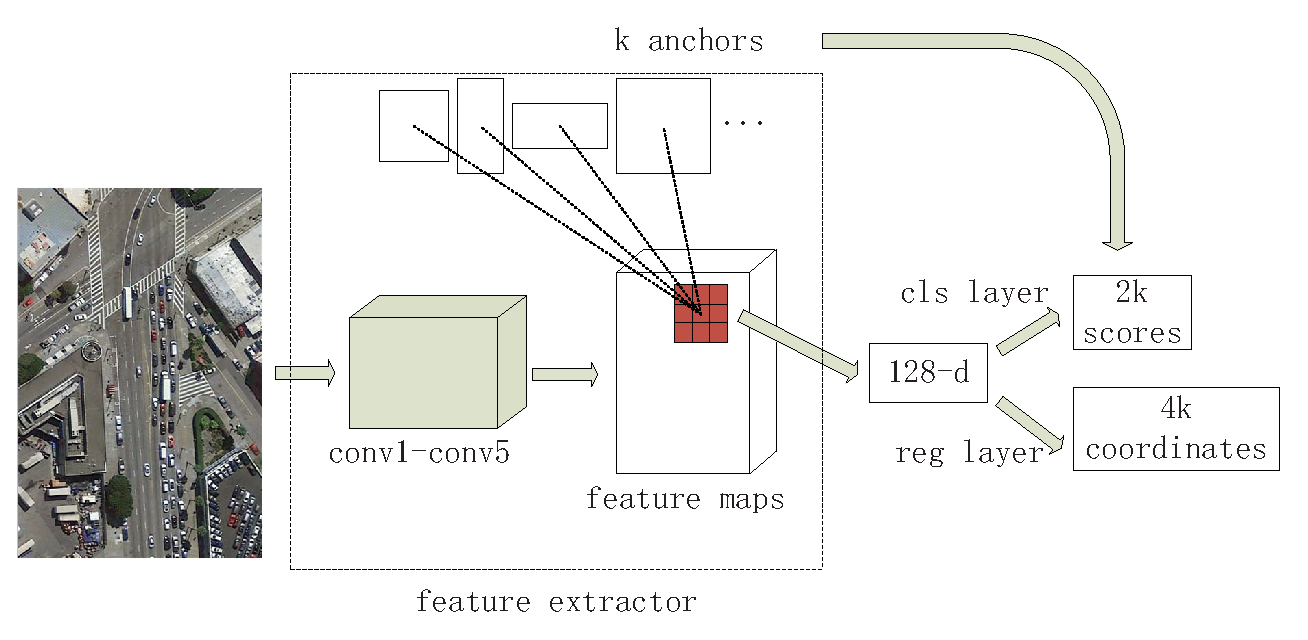
\includegraphics[height=5.0cm]{framework}
\caption{Our RPN-based detection framework. The input is a raw satellite image of 3 channels. A CNN of 5 convolution layers acts as a feature extractor. The two sibling parts, classification layer and regression layer do the following detection work. We use k anchors to hypothesize the vehicle locations}
\label{fig:example}
\end{figure}

\subsection{Architecture of RPN}

The architecture of RPN used in this paper is showed in figure 1. It consists of an feature extraction part and two sibling part--classification and regression. Our RPN model is acturally implemented as a fully-convolutional network\cite{fcn}. In our experiments we investigate Zeiler and Fergus's model\cite{zfnet} which has 5 convolutional layers. ZF-net is designed for the ILSVRC competition\cite{ilsvrc} which has 1000 categories. As for vehicle detection it is redundant. Moreover, vehicles in satellite images are quite different from natural objects for they occupy much less pixels. So we redesigned our DNN model. For clarity we demonstrate our DNN in table 1. Our model has the same depth with ZF-net but smaller width. In practice, we compared our "thiner" model with ZF-net model and found that our model which has much fewer parameters did not lose much accuracy while has much faster speed. 

\vspace{-3ex}

\setlength{\tabcolsep}{4pt}
\begin{table}
%\setlength{\abovecaptionskip}{-10pt}
%\setlength{\belowcaptionskip}{1pt}
\begin{center}
\caption{RPN configurations. For each convolutional layer ``parameters" gives the filter size and the stride which the filter is sliding with and ``filter numbers" gives the convolution kernel numbers of that layer. The pooling layers, LRN layers and ReLU activation layers are not shown for brevity}
\label{table:headings}
\begin{tabular}{ccccccccc}
\hline\noalign{\smallskip}
layer & conv1 & conv2 & conv3 & conv4 & conv5  & rpn\_conv1 & cls & reg \\
\noalign{\smallskip}
\hline
\noalign{\smallskip}
parameters  &  3$\times$3,2  &  3$\times$3,2  &  3$\times$3,1  &  3$\times$3,1  &  3$\times$3,1  &  3$\times$3,1 &  1$\times$1,1 &  1$\times$1,1 \\
filter numbers & 48 & 128 & 192 & 192 & 128 & 128 & 18 & 36 \\
\hline
\end{tabular}
\end{center}
\end{table}
\setlength{\tabcolsep}{200pt}

\vspace{-7ex}


\subsection{Learning methodology}
To narrow the vehicle object searching space, RPN uses several reference windows (anchors) instead of searching every scale and aspect ratio. At training stage, our RPN model takes a image of 3 channels as input and generates feature maps of 256 channels after layer conv5. So in each position (x,y) of those features maps we can extract a 128-dimensional vector corresponding to k anchors in the original image. If one anchor has intersection-over-union (IOU) overlap with any groundtruth box lager than a threshold we take it as a positive sample and similarly, if the IOU is less than another threshold we consider it as a negative sample. For anchors we use three 3 scales with boxes areas of 36$\times$36, 44$\times$44, and 50$\times$50 pixels, and 3 aspect ratios of 2:1,1:1, and 1:2. The 9 anchors we use are shown in table 2.

\vspace{-3ex}
\setlength{\tabcolsep}{4pt}
\begin{table}
\begin{center}
\caption{anchors }
\label{table:headings}
\begin{tabular}{ccccccccc}
\hline\noalign{\smallskip}
36$^{2}$,2:1 & 36$^{2}$,1:1 & 36$^{2}$,1:2 & 44$^{2}$,2:1 & 44$^{2}$,1:1 & 44$^{2}$,1:2 & 50$^{2}$,2:1 & 50$^{2}$,1:1 & 50$^{2}$,1:2\\
\noalign{\smallskip}
\hline
\noalign{\smallskip}
50$\times$26 & 36$\times$36 & 26$\times$50 & 62$\times$31 & 44$\times$44 & 31$\times$62 & 70$\times$36 & 50$\times$50 & 36$\times$70 \\
\hline
\end{tabular}
\end{center}
\end{table}
\setlength{\tabcolsep}{1.4pt}
\vspace{-5ex}

RPN as a fully-convolutional network\cite{fcn} is trained end-to-end by back-propagation(BP)\cite{lecun89} and the optimization scheme we use is stochastic gradient descent(SGD)\cite{lecun89}. We define our multi-task loss function following \cite{fast-rcnn}:
\begin{equation}
  \L(\left\{p_{i}\right\},\left\{t_{i}\right\}) = \frac{1}{N_{cls}}\sum_{i}L_{cls}(p_{i},p_{i}^{*})+\lambda\frac{1}{N_{reg}}
  \sum_{i}p_{i}^{*}L_{reg}(t_{i},t_{i}^{*})\ . 
\end{equation}
 Here, i is the index of anchors in a mini-batch and p$_{i}$ is the predicted probability of anchor i being an object. The corresponding ground-truth label of p$_{i}$ is p$_{i}^{*}$ which is 1 if the anchor is positive and 0 otherwise. Similarly, t$_{i}$ is the 4 predicted parameterized coordinates of the predicted bounding box and t$_{i}^{*}$ the ground-truth. The classification loss L$_{cls}$ is a vehicle vs. non-vehicle log loss and we use smooth function defined in \cite{fast-rcnn} for regression loss L$_{reg}$. 
We iterate 10000 times with learning rate 0.001 for the first 7000 mini-batches and 0.0001 for the next 3000 mini-batches on our training set. The momentum and weight decay we use are 0.9 and 0.0005 respectively\cite{alexnet}. Our implementation is based on Caffe\cite{caffe}----one of the most popular deep learning framework.




\section{Experiment}
This part dispatches details of our experiment results. Specificly, we first introduce our dataset and then we compare the detection accuracy of our method with that of some typical methods. Finally our method is compared to other DNN-based methods on the subject of speed.   
   
The dataset we use is that of \cite{xychen-hy} which includes 63 satellite images (1368$\times$972) from google earth of San Francisco city containing 6887 vehicle samples. To guarantee adequate training data, we split the dataset to 46 and 17 for training and testing randomly. At training stage, we augment the training set by rotating the images by 90$^{\circ}$, 180$^{\circ}$, 270$^{\circ}$ and flipping the images horizontally. No further data augmentation is done.

Here the false alarm rate (FAR), precision rate (PR), and recall rate(RR) are defined as 


\begin{equation} 
\left\{
\begin{aligned}
FAR & = & \frac{number \ of \ false \ alarms}{number \ of \ vehicles} & \times 100 \% \\
PR  & = & \frac{number \ of \ detected \ vehicles}{number \ of \ detected \ objects} & \times 100 \% \\
RR  & = & \frac{number \ of \ detected \ vehicles}{number \ of \ vehicles}& \times 100 \%
\end{aligned}
\ .
\right.
\end{equation}


\begin{table}% 加*表示跨栏,一般在双栏paper中使用
\begin{center}
\setlength{\abovecaptionskip}{-7pt}
\caption{FAR and processing time of our method and other methods on vehicle test set}
\label{table:headings}
{\begin{tabular}{|c|c|c|c|c|c|c|}% 列中文本左对齐,r:列中文本右对齐,c:列中文本居中
\hline
method & \multicolumn{6}{|c|}{give recall rate} \\
\cline{2-7}
 &\ 95\% & 90\% & 85\% & 80\% & 75\% & 70\% \\
\hline
Our & 22.8  & 12.1 & 7.43 & 5.26 & 3.57 & 2.92 \\
\hline
DNN & 23.5 & 12.2 & 7.5 & 5.07 & 3.45 & 2.61 \\
\hline
HOG+SVM\cite{hogsvm} & 67.5 & 43.4 & 29.3 & 20.2 & 14.3 & 10.3 \\
\hline
LBP+SVM\cite{lbpsvm} & 87.6  & 59.2 & 43.0 & 32.8 & 24.5 & 19.4 \\
\hline
Adaboost\cite{adaboost} & 91.6 & 65.3 & 49.1 & 40.1 & 31.6 & 25.8 \\
\hline
\multicolumn{7}{|c|}{test time for one image(s)} \\
\hline
\multicolumn{2}{|c|}{Ours} & \multicolumn{5}{|c|}{0.2}\\
\hline
\multicolumn{2}{|c|}{BING+CNN\cite{qushenquan}} & \multicolumn{5}{|c|}{0.7}\\
\hline
\multicolumn{2}{|c|}{HDNN\cite{xychen-hy}} & \multicolumn{5}{|c|}{8}\\
\hline
\end{tabular}}
\end{center}
\end{table}

In table 3, We list the FAR at given RR of our method and 4 other typical methods. Our method outperforms other methods at recall rate higher than 80$\%$. It means our detector is more robust for it can detect objects which are very hard for the rest methods and that proves the benefits of deep convolutional features and position regression. Moreover, the performance of our method at RR lower than 80$\%$ is also compelling. In fig. 2, we give some detection results samples. The testing images cover scenes from road with many trees to parking lot. Our detector performs very well even vehicle objects are quite dense on parking pot or sheltered by trees.


\begin{figure}
\centering
\includegraphics[height=5.5cm]{results}
\caption{Some detection results in San Francisco.The four images cover scenes from road with trees to parking lot}
\label{fig:example}
\end{figure}


Since our detection framework is designed to be a single-stage detector, it also has a very fast speed. In table 3, we give the processing time of one image of 3 DNN-based methods. Our detector achieves a frame rate of 5 fps on a computer with NVIDIA GTX960. There are two main reasons that our method is superior in speed. One is discarding proposal extraction stage which is an essential step of the rest methods and the other is that we do convolutions to the whole original image to extract features rather than one proposal by another. So for one testing image, our network does forward propagation only once while the other methods need to do it hundreds or thousands times depending on how many region proposals they extract in the region proposals extracting stage.



\section{Conclusion}
In this paper, we propose a new automatic satellite vehicle detection framework based on RPN. Different from traditional manual feature-based or DNN-based methods which are designed multi-stages, our method takes only one stage both in training and testing. By elaborating the RPN architecture and integrating several learning tricks, a very robust and real-time vehicle detector is obtained. Our experiment results show that our approach achieves better performance in both detection accuracy and speed in comparison to alternative approaches.

\bibliographystyle{splncs}
\bibliography{egbib}

\end{document}
